% C18 -- 19 de octubre de 2026.
% Fuentes: Pizarras recortadas/Screenshots C18/P01--P18.png; C18.txt.
% Se aclaran los índices F_{-n} y el carácter no literal de las inclusiones de conos.

Terminamos las propiedades formales de la categoría homotópica estable. Estudiaremos la compatibilidad del smash con los triángulos, la suspensión y la suma de morfismos; después construiremos la inclusión de Spanier--Whitehead y describiremos su imagen mediante espectros finitos. La propiedad de generación por el espectro esfera se reserva para la siguiente clase.

Denotamos el espectro esfera por $\mathbb S$. Salvo cuando trabajemos con modelos concretos, todos los productos smash de espectros se entienden derivados. Las construcciones con espacios se realizan con modelos CW bien punteados.

%%%%%%%%%%%%%%%%%%%%%%%%%%%%%%%%%%%%%%%%%%%%%%%%%%%%%%%%%%%%%%%%%%%%%%%%%%%%%%%
\section{Compatibilidad del smash con la estructura estable}
%%%%%%%%%%%%%%%%%%%%%%%%%%%%%%%%%%%%%%%%%%%%%%%%%%%%%%%%%%%%%%%%%%%%%%%%%%%%%%%

%%%%%%%%%%%%%%%%%%%%%%%%%%%%%%%%%%%%%%%%%%%%%%%%%%%%%%%%%%%%%%%%%%%%%%%%%%%%%%%
\subsection{Triángulos y producto derivado}
%%%%%%%%%%%%%%%%%%%%%%%%%%%%%%%%%%%%%%%%%%%%%%%%%%%%%%%%%%%%%%%%%%%%%%%%%%%%%%%
% P01--P03.
Ya conocemos la estructura aditiva de $\Ho(\Sp^{\mathbb N})$. Recordemos además dos resultados estructurales, que enunciamos sin demostrar todos sus axiomas.
\begin{teo}[Estructura de la categoría homotópica estable]\label{teo:c18-estructura}
La categoría $\Ho(\Sp^{\mathbb N})$ es triangulada. Sus triángulos distinguidos son los isomorfos a los triángulos de cofibra
\[
X\xlongrightarrow{f}Y\longrightarrow C_f\longrightarrow\Sigma X.
\]
Asimismo, el smash derivado le da una estructura monoidal simétrica cerrada con unidad $\mathbb S$.
\end{teo}
\begin{nota}
La estructura monoidal se remonta a Adams; véanse \cite{adams1974} y \cite[capítulos~3 y~4]{malkiewich}. Aquí verificamos las compatibilidades necesarias, sin desarrollar la construcción completa del smash de Adams ni todos los axiomas de triangulación. Un morfismo de $\Ho(\Sp^{\mathbb N})$ puede estar representado por un zigzag; el enunciado no exige que el triángulo venga inicialmente dado por un solo morfismo estricto de espectros.
\end{nota}

\begin{prop}\label{prop:c18-smash-exacto}
Para cada espectro $Z$, el funtor $Z\wedge^L-$ preserva los triángulos distinguidos.
\end{prop}
\begin{proof}
Consideremos primero un espacio punteado $K$. Como $K\wedge-$ es adjunto izquierdo, preserva pushouts. Usando $I_+$ para el intervalo con punto base disjunto y colapsando el extremo que forma el vértice del cono, obtenemos la identificación natural
\[
C_{1_K\wedge f}\cong
\bigl(K\wedge CX\bigr)\cup_{1\wedge f}(K\wedge Y)
\cong K\wedge(CX\cup_fY)=K\wedge C_f.
\]
Para espectros, elijamos la misma sucesión de índices en todos los productos de Adams. Si $p_r+q_r=r$, entonces
\[
\begin{aligned}
(C_{1_Z\wedge f})_r
&=(Z_{p_r}\wedge CX_{q_r})\cup_{1\wedge f_{q_r}}
  (Z_{p_r}\wedge Y_{q_r})\\
&\cong Z_{p_r}\wedge(CX_{q_r}\cup_{f_{q_r}}Y_{q_r})
=(Z\wedge C_f)_r.
\end{aligned}
\]
La naturalidad de los pushouts hace compatibles estas identificaciones con los morfismos estructurales. Así, para modelos cofibrantes, las dos filas del diagrama representan sucesiones cofibradas:
\[
\begin{tikzcd}[column sep=large]
X\arrow[r,"f"]&Y\arrow[r]&C_f\\
Z\wedge X\arrow[r,"1\wedge f"]&Z\wedge Y\arrow[r]&Z\wedge C_f.
\end{tikzcd}
\]
Para pasar al producto derivado, usamos el reemplazo cofibrante functorial $Q$ y comparamos las sucesiones de cofibra correspondientes a $f$ y a $Qf$:
\[
\begin{tikzcd}[column sep=large,row sep=large]
X\arrow[r,"f"]&Y\arrow[r]&C_f\\
QX\arrow[r,"Qf"]\arrow[u,"\simeq"]&QY\arrow[r]\arrow[u,"\simeq"]&C_{Qf}\arrow[u,"\simeq"] .
\end{tikzcd}
\]
La tercera flecha es equivalencia estable por las sucesiones exactas largas de la clase~17 y el lema de los cinco. Aplicamos ahora el cálculo anterior a
\[
QZ\wedge QX\longrightarrow QZ\wedge QY\longrightarrow QZ\wedge C_{Qf}.
\]
Esta sucesión representa, en $\Ho(\Sp^{\mathbb N})$, la fila
\[
Z\wedge^L X\longrightarrow Z\wedge^L Y\longrightarrow Z\wedge^L C_f.
\]
El mapa de conexión se obtiene del colapso del cono y de la identificación natural con la suspensión que veremos enseguida. Por ello también se conserva el cuarto término del triángulo. Los triángulos isomorfos a estos se preservan por functorialidad.
\end{proof}

%%%%%%%%%%%%%%%%%%%%%%%%%%%%%%%%%%%%%%%%%%%%%%%%%%%%%%%%%%%%%%%%%%%%%%%%%%%%%%%
\subsection{Suspensión, unidad y coproductos}
%%%%%%%%%%%%%%%%%%%%%%%%%%%%%%%%%%%%%%%%%%%%%%%%%%%%%%%%%%%%%%%%%%%%%%%%%%%%%%%
% P04--P05.
Hay un isomorfismo natural en $\Ho(\Sp^{\mathbb N})$
\[
\sigma_{X,Y}\colon (\Sigma X)\wedge^L Y\xrightarrow{\cong}
\Sigma(X\wedge^L Y).
\]
En un modelo de Adams está inducido por la reasociación de
$(S^1\wedge X_{p_r})\wedge Y_{q_r}$ con
$S^1\wedge(X_{p_r}\wedge Y_{q_r})$. También se obtiene asociando el smash con el espectro de suspensión de $S^1$:
\[
(\Sigma^\infty S^1\wedge^L X)\wedge^L Y
\cong\Sigma^\infty S^1\wedge^L(X\wedge^L Y).
\]
Para un espacio punteado $K$, se tiene
\[
\Sigma^\infty K\wedge^L X\simeq K\wedge X
\]
con los reemplazos apropiados. Adams justifica este cálculo ampliando los modelos de smash: se particiona $\mathbb N=B\amalg C$, permitiendo que la coordenada correspondiente al espectro de suspensión permanezca fija y que la otra tienda a infinito. Los distintos modelos se comparan mediante un telescopio común, que denotamos $\operatorname{hocolim}\mathcal D$:
\[
\begin{tikzcd}[column sep=large]
X\wedge_{B,C}Y\arrow[r,"\simeq"]&\operatorname{hocolim}\mathcal D
&X\wedge_{B',C'}Y\arrow[l,"\simeq"'] .
\end{tikzcd}
\]
Cuando $X=\Sigma^\infty K$, el segundo modelo puede tener $B'$ finito y $C'$ infinito; entonces sus niveles se calculan como $K\wedge Y_r$. Esta posibilidad no se afirma para espectros arbitrarios. Solo utilizamos la función de este telescopio comparador, sin construirlo por completo.

La compatibilidad de $\sigma$ con la unidad se expresa por el triángulo
\[
\begin{tikzcd}[column sep=large,row sep=large]
(\Sigma X)\wedge^L\mathbb S\arrow[d,"\sigma_{X,\mathbb S}"']\arrow[dr,"\rho_{\Sigma X}"]&\\
\Sigma(X\wedge^L\mathbb S)\arrow[r,"\Sigma\rho_X"']&\Sigma X.
\end{tikzcd}
\]
En el modelo que deja fija la coordenada del espectro esfera, $\rho_Y$ es el homeomorfismo $Y_r\wedge S^0\cong Y_r$. El triángulo anterior se reduce, nivel a nivel, a
\[
\begin{tikzcd}[column sep=large,row sep=large]
(S^1\wedge X_r)\wedge S^0\arrow[d,"\alpha"']\arrow[dr,"\cong"]&\\
S^1\wedge(X_r\wedge S^0)\arrow[r,"\cong"']&S^1\wedge X_r.
\end{tikzcd}
\]
Ambos caminos envían la clase de $(s,x,1)$ a la de $(s,x)$; por tanto conmutan. Para cualquier otro modelo, esta igualdad se transporta a $\Ho(\Sp^{\mathbb N})$ por las equivalencias de comparación.

\begin{ejer}\label{ejer:c18-smash-coproductos}
Probar que el smash derivado preserva coproductos arbitrarios:
\[
X\wedge^L\Bigl(\bigvee_{j\in J}Y_j\Bigr)
\cong\bigvee_{j\in J}(X\wedge^L Y_j).
\]
\end{ejer}
\begin{sol}
La estructura cerrada del \myref{teo:c18-estructura} da un adjunto derecho $\ihom(X,-)$ en $\Ho(\Sp^{\mathbb N})$. Para cualquier $T$, la adjunción y la propiedad universal del coproducto dan biyecciones naturales
\[
\begin{aligned}
[X\wedge^L(\bigvee_jY_j),T]_s
&\cong[\bigvee_jY_j,\ihom(X,T)]_s\\
&\cong\prod_j[Y_j,\ihom(X,T)]_s\\
&\cong\prod_j[X\wedge^L Y_j,T]_s.
\end{aligned}
\]
Esto es precisamente la propiedad universal del coproducto de los objetos $X\wedge^L Y_j$. La comparación inducida por las inclusiones de cada $Y_j$ es, por tanto, un isomorfismo. Por simetría ocurre lo mismo en la otra variable. Si se usan modelos, deben tomarse coproductos de reemplazos cofibrantes: la afirmación pertenece a $\Ho(\Sp^{\mathbb N})$, no a cualquier elección de productos sin derivar.
\end{sol}

%%%%%%%%%%%%%%%%%%%%%%%%%%%%%%%%%%%%%%%%%%%%%%%%%%%%%%%%%%%%%%%%%%%%%%%%%%%%%%%
\section{Bilinealidad del producto de morfismos}
%%%%%%%%%%%%%%%%%%%%%%%%%%%%%%%%%%%%%%%%%%%%%%%%%%%%%%%%%%%%%%%%%%%%%%%%%%%%%%%
% P06--P07.
\begin{prop}
El mapa inducido por el smash
\[
[X,Y]_s\times[Z,W]_s\longrightarrow[X\wedge^L Z,Y\wedge^L W]_s,
\qquad ([f],[g])\longmapsto[f\wedge^L g],
\]
es bilineal.
\end{prop}
\begin{proof}
Omitimos el superíndice $L$ dentro de esta demostración. Sean $f,f'\colon X\to Y$ y $g\colon Z\to W$ morfismos de $\Ho(\Sp^{\mathbb N})$. En la clase~17 se probó que
\[
f+f'=\nabla_Y(f\vee f')a_X^{-1}\Delta_X,
\qquad a_X\colon X\vee X\xrightarrow{\cong}X\times X.
\]
Comencemos con el siguiente diagrama:
\[
\begin{tikzcd}[column sep=large,row sep=large]
&X\vee X\arrow[r,"f\vee f'"]\arrow[d,"a_X"]&Y\vee Y\arrow[r,"\nabla_Y"]&Y\\
X\arrow[r,"\Delta_X"']&X\times X&&
\end{tikzcd}
\]
Escribamos $U=X\wedge Z$, $V=Y\wedge W$ y $d$ para las distribuciones sobre coproductos del ejercicio anterior. La parte central y las comparaciones del diagrama ampliado son
\[
\begin{tikzcd}[column sep=4em,row sep=2.4em]
&U\vee U\arrow[rr,"(f\wedge g)\vee(f'\wedge g)"]&&V\vee V\arrow[dr,"\nabla_V"]&\\
&(X\vee X)\wedge Z\arrow[u,"d","\cong"']\arrow[rr,"(f\vee f')\wedge g"]\arrow[d,"a_X\wedge1"']
&&(Y\vee Y)\wedge W\arrow[u,"d","\cong"']\arrow[r,"\nabla_Y\wedge1"']&V\\
U\arrow[r,"\Delta_X\wedge1"]\arrow[rr,bend right=25,"\Delta_U"']&(X\times X)\wedge Z\arrow[r,"c"]&U\times U&&
\arrow[from=1-2,to=3-3,rojoDiagramaCIMAT,"a_U"{pos=.8},"\cong"'{pos=.8},crossing over]
\end{tikzcd}
\]
Aquí $c$ tiene componentes $p_1\wedge1$ y $p_2\wedge1$. Comprobemos explícitamente las conmutatividades. Las inclusiones $i_1,i_2$ de $X$ satisfacen $p_ri_s=1$ para $r=s$ y $p_ri_s=0$ para $r\ne s$. Por ello
\[
c(a_X\wedge1)=a_Ud,
\qquad c(\Delta_X\wedge1)=\Delta_U.
\]
La primera identidad se verifica precomponiendo con cada inclusión del coproducto, y la segunda componiendo con cada proyección. Además, $a_X\wedge1$, $a_U$ y $d$ son isomorfismos; la primera identidad prueba que también lo es $c$. La naturalidad de $d$ da el cuadrado superior, y la igualdad del triángulo derecho se verifica en cada sumando, donde ambos caminos son la identidad de $V$. En consecuencia,
\[
\begin{aligned}
(f+f')\wedge g
&=\nabla_V\bigl((f\wedge g)\vee(f'\wedge g)\bigr)a_U^{-1}\Delta_U\\
&=(f\wedge g)+(f'\wedge g).
\end{aligned}
\]
La misma comprobación en la otra variable prueba la otra distributividad. Los morfismos cero se preservan porque se factorizan por el objeto cero, cuyo smash es cero. Esto completa la bilinealidad, incluidos los inversos aditivos.
\end{proof}

%%%%%%%%%%%%%%%%%%%%%%%%%%%%%%%%%%%%%%%%%%%%%%%%%%%%%%%%%%%%%%%%%%%%%%%%%%%%%%%
\section{La inclusión de Spanier--Whitehead}
%%%%%%%%%%%%%%%%%%%%%%%%%%%%%%%%%%%%%%%%%%%%%%%%%%%%%%%%%%%%%%%%%%%%%%%%%%%%%%%

%%%%%%%%%%%%%%%%%%%%%%%%%%%%%%%%%%%%%%%%%%%%%%%%%%%%%%%%%%%%%%%%%%%%%%%%%%%%%%%
\subsection{Objetos, adjunciones y cálculo de morfismos}
%%%%%%%%%%%%%%%%%%%%%%%%%%%%%%%%%%%%%%%%%%%%%%%%%%%%%%%%%%%%%%%%%%%%%%%%%%%%%%%
% P07--P09.
Para $X$ un CW complejo finito punteado, definimos
\[
\iota\colon\SW\longrightarrow\Ho(\Sp^{\mathbb N}),
\qquad (X,n)\longmapsto\sh^n\Sigma^\infty X=:F_{-n}X.
\]
La asignación de objetos y de morfismos se expresa en el diagrama:
\[
\begin{tikzcd}[column sep=huge,row sep=large]
(X,n)\arrow[r,mapsto]\arrow[d,"{[f]}"']&F_{-n}X\arrow[d,"{\iota([f])}"]\\
(Y,m)\arrow[r,mapsto]&F_{-m}Y.
\end{tikzcd}
\]
El signo del índice importa: el espectro libre $F_rX$ de la clase~11 coloca $X$ en el nivel $r$, de modo que aquí aparece $F_{-n}$.
\begin{nota}\label{nota:c18-indices}
En espectros secuenciales, la adjunción estricta de $F_r$ con la evaluación en $r$ se aplica a $r\ge0$. Para usarla podemos reemplazar $(X,n)$ por la pareja isomorfa $(\Sigma^tX,n-t)$ y hacer no positivos los enteros de las parejas que intervienen. Después se transporta el resultado mediante esos isomorfismos. Las expresiones con niveles negativos de la pizarra se interpretan de este modo, o como fórmulas válidas en una cola cofinal; no se evalúa literalmente un espectro secuencial en un nivel negativo.
\end{nota}
Sea $R$ el reemplazo por un $\Omega$-espectro construido mediante telescopios y $\eta\colon1\to R$ su equivalencia estable natural. Para $n,m\le0$, las adjunciones y la finitud de $X$ proporcionan
\[
\begin{aligned}
[F_{-n}X,F_{-m}Y]_s
&\cong[F_{-n}X,RF_{-m}Y]_s\\
&\cong[F_{-n}X,RF_{-m}Y]_h\\
&\cong[X,(RF_{-m}Y)_{-n}]_*\\
&\cong\varinjlim\nolimits_a[X,\Omega^a(F_{-m}Y)_{-n+a}]_*\\
&\cong\varinjlim\nolimits_a[\Sigma^aX,(F_{-m}Y)_{-n+a}]_*\\
&\cong\varinjlim\nolimits_a[\Sigma^aX,\Sigma^{m-n+a}Y]_*\\
&\cong\varinjlim\nolimits_k[\Sigma^{n+k}X,\Sigma^{m+k}Y]_*\\
&=\hom_{\SW}((X,n),(Y,m)).
\end{aligned}
\]
La penúltima biyección usa $a=n+k$ y se toma en la cola donde los exponentes son no negativos. El término de telescopio que interviene es
\[
(RF_{-m}Y)_{-n}=\operatorname{hocolim}_{a\ge0}
\Omega^a(F_{-m}Y)_{-n+a}.
\]
El sistema del telescopio se dibuja explícitamente como
\[
\begin{tikzcd}[column sep=1.8em]
(F_{-m}Y)_{-n}\arrow[r]&\Omega(F_{-m}Y)_{-n+1}\arrow[r]
&\Omega^2(F_{-m}Y)_{-n+2}\arrow[r]&\cdots .
\end{tikzcd}
\]
Como $X$ es un CW complejo finito, una aplicación desde $X$ y una homotopía desde $X\wedge I_+$ tienen imagen en un subtelescopio finito. Este se retrae por deformación sobre su última etapa. Así se justifican tanto la sobreyectividad como la inyectividad al pasar al colímite de clases. Es el cálculo de \cite[Corolario~3.2.2.2 y Proposición~4.2.2.1]{malkiewich}.

Para describir la biyección inversa, tomemos
$f\colon\Sigma^{n+k}X\to\Sigma^{m+k}Y$. Su adjunto seguido de la inclusión de etapa es
\[
f^\perp\colon X\longrightarrow\Omega^{n+k}\Sigma^{m+k}Y
\longrightarrow(RF_{-m}Y)_{-n}.
\]
La adjunción libre da un único mapa estricto
$(f^\perp)^{\perp'}\colon F_{-n}X\to RF_{-m}Y$ con componente $f^\perp$ en el nivel $-n$. Por tanto, el morfismo asociado está representado por
\[
\begin{tikzcd}[column sep=huge]
F_{-n}X\arrow[r,"(f^\perp)^{\perp'}"]&RF_{-m}Y&F_{-m}Y\arrow[l,"\eta_{F_{-m}Y}"',"\simeq"] .
\end{tikzcd}
\]
En particular, $\iota([f])=\eta_{F_{-m}Y}^{-1}(f^\perp)^{\perp'}$ en $\Ho(\Sp^{\mathbb N})$.

%%%%%%%%%%%%%%%%%%%%%%%%%%%%%%%%%%%%%%%%%%%%%%%%%%%%%%%%%%%%%%%%%%%%%%%%%%%%%%%
\subsection{Suspensión de representantes y composición}
%%%%%%%%%%%%%%%%%%%%%%%%%%%%%%%%%%%%%%%%%%%%%%%%%%%%%%%%%%%%%%%%%%%%%%%%%%%%%%%
% P10--P13. Esquema reutilizado para las ilustraciones de telescopios.
% Geometría adaptada de RE_C10: tapas, arcos ocultos y cilindros contiguos.
% Las superficies son esquemáticas; no representan inclusiones de espacios.
\newcommand{\cXVIIItapaDerecha}[3]{%
  \draw[dashed] (#1,#3) arc[start angle=90,end angle=270,
    x radius=#2,y radius=#3];
  \draw (#1,#3) arc[start angle=90,end angle=-90,
    x radius=#2,y radius=#3];}
\newcommand{\cXVIIItapaIzquierda}[4]{%
  \pgfmathsetmacro{\anguloOculto}{asin(#4/#3)}
  \draw (#1,#3) arc[start angle=90,end angle={180-\anguloOculto},
    x radius=#2,y radius=#3];
  \draw[dashed] ({#1-#2*cos(\anguloOculto)},#4)
    arc[start angle={180-\anguloOculto},end angle={180+\anguloOculto},
    x radius=#2,y radius=#3];
  \draw ({#1-#2*cos(\anguloOculto)},{-#4})
    arc[start angle={180+\anguloOculto},end angle=450,
    x radius=#2,y radius=#3];}
% Cono de eje horizontal: vértice a la izquierda y base elíptica a la derecha.
\newcommand{\cXVIIIcono}[3]{%
  \draw (-#1,0)--(0,#3) (-#1,0)--(0,-#3);
  \cXVIIItapaDerecha{0}{#2}{#3}}
% El parámetro 1 añade el cono inicial; 0 deja la tapa visible.
\newcommand{\cXVIIItubo}[1]{%
  \draw (0,.32)--(1.5,.32) (0,-.32)--(1.5,-.32);
  \ifnum#1=1 \cXVIIIcono{1.05}{.10}{.32}
  \else \draw (0,0) ellipse[x radius=.10,y radius=.32];\fi
  \cXVIIItapaDerecha{1.5}{.10}{.32}
  \draw (1.5,.60)--(3.3,.60) (1.5,-.60)--(3.3,-.60);
  \cXVIIItapaIzquierda{1.5}{.16}{.60}{.32}
  \cXVIIItapaDerecha{3.3}{.16}{.60}
  \draw (3.3,.90)--(5.1,.90) (3.3,-.90)--(5.1,-.90);
  \cXVIIItapaIzquierda{3.3}{.23}{.90}{.60}
  \draw[dotted] (5.1,.90)--(5.8,.90) (5.1,-.90)--(5.8,-.90);}

\newcommand{\cXVIIIsuspension}{%
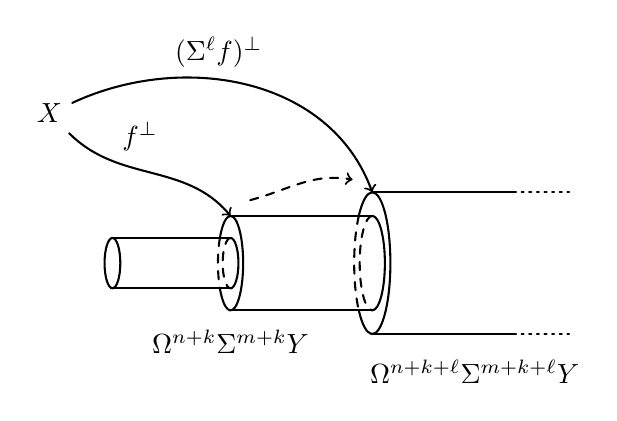
\begin{tikzpicture}[x=1cm,y=1cm,line width=.75pt,line cap=round,
                    line join=round,baseline=(current bounding box.center)]
  \cXVIIItubo{0}
  \node (x) at (-.8,1.9) {$X$};
  \draw[->] (x) to[out=-45,in=130] (1.5,.60);
  \node at (.35,1.61) {$f^\perp$};
  \draw[->] (x) to[out=25,in=110] (3.3,.90);
  \node at (1.35,2.68) {$(\Sigma^\ell f)^\perp$};
  \draw[->,dashed] (1.75,.80) to[out=15,in=170] (3.05,1.06);
  \node[below] at (1.5,-.72) {$\Omega^{n+k}\Sigma^{m+k}Y$};
  \node[below] at (4.6,-1.10) {$\Omega^{n+k+\ell}\Sigma^{m+k+\ell}Y$};
\end{tikzpicture}}

\newcommand{\cXVIIIdoble}{%
\begin{tikzpicture}[x=.80cm,y=.80cm,line width=.75pt,line cap=round,
                    line join=round,baseline=(current bounding box.center)]
  \begin{scope}[shift={(-6.8,0)},scale=.65]
    \cXVIIItubo{0}
    \draw[rojoDiagramaCIMAT] (0,0) ellipse[x radius=.10,y radius=.32];
    \node at (2.4,1.6) {$(RB)_j$};
  \end{scope}
  % Cilindro exterior: sus generatrices rojas conectan las dos etapas.
  \draw[rojoDiagramaCIMAT,->] (.05,1.7)--(.65,-1.7);
  \draw[rojoDiagramaCIMAT,->] (5.1,1.7)--(5.7,-1.7);
  \begin{scope}[shift={(0,1.7)}]
    \fill[yellow!20] (0,-.32)--(1.5,-.32)--(1.5,-.60)
      --(3.3,-.60)--(3.3,-.90)--(5.1,-.90)--(5.1,.90)
      --(3.3,.90)--(3.3,.60)--(1.5,.60)--(1.5,.32)--(0,.32)--cycle;
    \cXVIIItubo{0}
  \end{scope}
  \begin{scope}[shift={(.6,-1.7)}]\cXVIIItubo{0}\end{scope}
  \draw[->] (-6.8,.23) to[out=80,in=180] (-.15,1.7);
  \node at (-3.1,2.29) {$k'_j$};
  \draw[->] (-5.8,-.42) to[out=-60,in=180] (.43,-1.7);
  \node at (-2.8,-2.37) {$\Omega k'_{j+1}$};
  \node at (2.8,3.05) {$(RRC)_j$};
  \node[right] at (6,1.7) {$(RC)_j$};
  \node[right] at (6.6,-1.7) {$\Omega(RC)_{j+1}$};
  \node at (3.2,-3.15) {$\vdots$};
\end{tikzpicture}}

\newcommand{\cXVIIIconos}{%
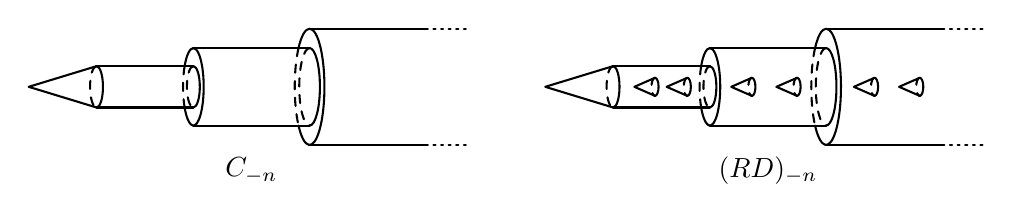
\begin{tikzpicture}[x=.82cm,y=.82cm,line width=.75pt,line cap=round,
                    line join=round,baseline=(current bounding box.center)]
  \cXVIIItubo{1}
  \node at (2.4,-1.30) {$C_{-n}$};
  \begin{scope}[shift={(8,0)}]
    \cXVIIItubo{1}
    % Conos en el interior de cada cilindro, sin cortar las tapas de unión.
    \foreach \x in {.65,1.15,2.15,2.85,4.05,4.75}{
      \begin{scope}[shift={(\x,0)}]
        \cXVIIIcono{.32}{.055}{.14}
      \end{scope}}
    \node at (2.4,-1.30) {$(RD)_{-n}$};
  \end{scope}
\end{tikzpicture}}

Si sustituimos $f$ por $\Sigma^\ell f$, obtenemos el triángulo homotópicamente conmutativo
\[
\begin{tikzcd}[column sep=large,row sep=large]
X\arrow[r,"f^\perp"]\arrow[dr,"(\Sigma^\ell f)^\perp"']
&\Omega^{n+k}\Sigma^{m+k}Y\arrow[d,"u^\ell"]\\
&\Omega^{n+k+\ell}\Sigma^{m+k+\ell}Y.
\end{tikzcd}
\]
Las dos etapas se incluyen en el mismo telescopio. Los cilindros de las aplicaciones estructurales realizan la homotopía entre ambas inclusiones compuestas. Su forma geométrica se conserva en el esquema
\[
\csname cXVIIIsuspension\endcsname
\]
Esto explica geométricamente la independencia del representante suspendido; la independencia de homotopías ya forma parte de las biyecciones anteriores.

Sean ahora $f\colon\Sigma^{n+k}X\to\Sigma^{m+k}Y$ y
$g\colon\Sigma^{m+\ell}Y\to\Sigma^{b+\ell}Z$. Para componer sus clases en $\SW$, suspendemos ambos mapas hasta una etapa común y obtenemos el representante
\[
\Sigma^kg\circ\Sigma^\ell f\colon
\Sigma^{n+k+\ell}X\longrightarrow\Sigma^{b+k+\ell}Z.
\]
La composición de sus imágenes está representada por el zigzag:
\[
\begin{tikzcd}[column sep=1.8em]
F_{-n}X\arrow[r,"h"]&RF_{-m}Y&F_{-m}Y\arrow[l,"\eta"',"\simeq"]\arrow[r,"k'"]&RF_{-b}Z&F_{-b}Z\arrow[l,"\eta"',"\simeq"]
\end{tikzcd}
\]
Aquí $h=((\Sigma^\ell f)^\perp)^{\perp'}$ y
$k'=((\Sigma^kg)^\perp)^{\perp'}$. Para no confundir $k'$ con el índice de suspensión, primero hagamos el cálculo formal con $A=F_{-n}X$, $B=F_{-m}Y$ y $C=F_{-b}Z$:
\[
\begin{tikzcd}[column sep=large,row sep=large]
A\arrow[r,"h"]&RB&B\arrow[l,"\eta_B"',"\simeq"]\arrow[r,"k'"]\arrow[d,"\eta_B"']&RC\arrow[d,"\eta_{RC}","\simeq"']&C\arrow[l,"\eta_C"',"\simeq"]\\
&&RB\arrow[r,"Rk'"']&RRC&
\end{tikzcd}
\]
La naturalidad de $\eta$ hace conmutar el cuadrado, y cancelamos las dos apariciones inversas de $\eta_B$. El zigzag resultante es
\[
\begin{tikzcd}[column sep=large]
A\arrow[r,"Rk'\circ h"]&RRC&RC\arrow[l,"\eta_{RC}"',"\simeq"]&C\arrow[l,"\eta_C"',"\simeq"] .
\end{tikzcd}
\]
% P12--P13; transcripción unificada 01:07:42--01:21:18.
Para identificar este zigzag con la imagen de la composición, describamos geométricamente el mapa $Rk'$. Fijemos un nivel $j$. El espacio $(RB)_j$ es un telescopio, mientras que $(RRC)_j$ es un telescopio de telescopios: el primero es $(RC)_j$, el siguiente corresponde a $\Omega(RC)_{j+1}$ y así sucesivamente. En el dibujo, los telescopios interiores se extienden horizontalmente; los cilindros exteriores, señalados en rojo, conectan uno con el siguiente.

En la primera etapa del telescopio de origen aplicamos $k'_j$. Como $k'=((\Sigma^kg)^\perp)^{\perp'}$, su construcción lleva esa etapa a una etapa del telescopio amarillo y después la incluye en él. Al aplicar $R$ a $k'$, la siguiente etapa se envía mediante $\Omega k'_{j+1}$ al segundo telescopio. En general, la aplicación sobre la etapa $a$ es
\[
\Omega^a B_{j+a}\xrightarrow{\Omega^a k'_{j+a}}
\Omega^a(RC)_{j+a}\longrightarrow(RRC)_j.
\]
Así, al avanzar por las etapas del origen, la imagen avanza dentro de los telescopios interiores y también pasa de un telescopio al siguiente. Este es el recorrido \emph{diagonal}:
\[
\csname cXVIIIdoble\endcsname
\]
La comparación consiste en efectuar esas mismas aplicaciones, con las suspensiones necesarias, pero avanzando siempre dentro del primer telescopio, el amarillo. Este mapa es $\varphi\colon RB\to RC$: en clase se lo llamó inicialmente $h$ y después se cambió a $\varphi$ para distinguirlo del mapa $h\colon A\to RB$. Al incluir su imagen en el telescopio doble obtenemos $\eta_{RC}\varphi$, pues $\eta_{RC}$ es precisamente la inclusión de la primera etapa exterior.

Ahora se comparan ambos recorridos. Sobre la primera etapa del origen ya coinciden. Para la segunda, se lleva la imagen de $\eta_{RC}\varphi$ desde el telescopio amarillo hasta el segundo, recorriendo el cilindro exterior que los une. Para la tercera se avanza hasta el tercero, y así sucesivamente. Los cilindros entre etapas del origen permiten interpolar entre estos recorridos: sus extremos se pegan mediante las aplicaciones estructurales con las que se ha construido $Rk'$. De este modo, el recorrido que permanece en el primer telescopio se deforma al recorrido diagonal. Esta homotopía geométrica da
\[
\eta_{RC}\circ\varphi\simeq Rk'.
\]
\begin{nota}
El profesor corrigió el sentido de esta construcción durante la explicación. Primero propuso llevar el mapa diagonal hacia el primer telescopio, pero los pegados pueden identificar puntos y no permiten invertir ese movimiento. La deformación se construye desde $\eta_{RC}\varphi$ hacia $Rk'$, avanzando por los cilindros rojos. Se obtiene una factorización de $Rk'$ \emph{salvo homotopía}; no se está afirmando una igualdad estricta de aplicaciones ni una retracción del telescopio doble sobre el primero.
\end{nota}
La homotopía permite reemplazar $Rk'\circ h$ por $\eta_{RC}\circ\varphi\circ h$ en el zigzag:
\[
\begin{tikzcd}[column sep=2em]
A\arrow[r,"h"]&RB\arrow[r,"\varphi"]&RC\arrow[r,"\eta_{RC}","\simeq"']&RRC&RC\arrow[l,"\eta_{RC}"',"\simeq"]&C\arrow[l,"\eta_C"',"\simeq"] .
\end{tikzcd}
\]
Las dos flechas con etiqueta $\eta_{RC}=\eta_{RF_{-b}Z}$ se recorren en sentidos opuestos y se cancelan en $\Ho(\Sp^{\mathbb N})$. El zigzag se reduce a
\[
\begin{tikzcd}[column sep=huge]
F_{-n}X\arrow[r,"\varphi\circ h"]&RF_{-b}Z&F_{-b}Z\arrow[l,"\eta_{F_{-b}Z}"',"\simeq"] .
\end{tikzcd}
\]
Para reconocer el primer mapa, volvamos al nivel $-n$, que determina un morfismo desde el espectro libre $F_{-n}X$. Primero, $h$ aplica el adjunto de $\Sigma^\ell f$ e incluye el resultado en una etapa del telescopio de $Y$. Después, $\varphi$ aplica allí el mapa correspondiente a $\Sigma^kg$, manteniendo el resultado dentro del primer telescopio de $Z$. Como los representantes se suspendieron hasta una etapa común, esto es aplicar sucesivamente $\Sigma^\ell f$ y $\Sigma^kg$, tomar el adjunto e incluirlo en el telescopio de $Z$. Por la adjunción libre, el mapa obtenido representa
\[
\varphi\circ h\simeq
\bigl((\Sigma^kg\circ\Sigma^\ell f)^\perp\bigr)^{\perp'}.
\]
El zigzag reducido es, pues, el que define la imagen de la composición. Concluimos que
\[
\iota([g])\iota([f])=\iota([\Sigma^kg\circ\Sigma^\ell f]).
\]

\begin{ejer}
Comprobar que $\iota$ envía la identidad a la identidad.
\end{ejer}
\begin{sol}
Tras el cambio de representante explicado al introducir los índices, podemos suponer $n\le0$. Representamos la identidad mediante $1_X$ en la etapa $k=-n$. Su primer adjunto es la identidad de $X$, seguida de la inclusión inicial $X\to(RF_{-n}X)_{-n}$. El adjunto libre de esa inclusión es precisamente $\eta_{F_{-n}X}$. Por consiguiente,
\[
\iota([1_X])=\eta_{F_{-n}X}^{-1}\eta_{F_{-n}X}=1_{F_{-n}X}.
\]
Para cualquier otra etapa, la compatibilidad con suspensión ya probada da el mismo resultado. Transportar a una pareja isomorfa no altera la identidad.
\end{sol}
Hemos probado que $\iota$ es un funtor y que es plenamente fiel, pues sus aplicaciones en los conjuntos de morfismos son las biyecciones calculadas antes.

%%%%%%%%%%%%%%%%%%%%%%%%%%%%%%%%%%%%%%%%%%%%%%%%%%%%%%%%%%%%%%%%%%%%%%%%%%%%%%%
\section{Triángulos, estructura monoidal y espectros finitos}
%%%%%%%%%%%%%%%%%%%%%%%%%%%%%%%%%%%%%%%%%%%%%%%%%%%%%%%%%%%%%%%%%%%%%%%%%%%%%%%

%%%%%%%%%%%%%%%%%%%%%%%%%%%%%%%%%%%%%%%%%%%%%%%%%%%%%%%%%%%%%%%%%%%%%%%%%%%%%%%
\subsection{Compatibilidad con los triángulos}
%%%%%%%%%%%%%%%%%%%%%%%%%%%%%%%%%%%%%%%%%%%%%%%%%%%%%%%%%%%%%%%%%%%%%%%%%%%%%%%
% P13--P16.
Un triángulo distinguido de $\SW$ es isomorfo, tras suspender un representante, a uno de la forma
\[
(X,n)\xrightarrow{[f]}(Y,n)\longrightarrow(C_f,n)\longrightarrow(X,n+1),
\qquad f\colon X\to Y.
\]
Pongamos $A=F_{-n}X$, $B=F_{-n}Y$, $D=F_{-n}C_f$ y $\gamma=\eta_BF_{-n}f$. El cambio de modelos se expresa como
\[
\begin{tikzcd}[column sep=1.5em,row sep=large]
A\arrow[r,"{\iota([f])}"]\arrow[d,equal]&B\arrow[r]\arrow[d,"\eta_B","\simeq"']&D\arrow[r]\arrow[d,"\eta_D","\simeq"']&F_{-(n+1)}X\arrow[d,"\eta","\simeq"']\\
A\arrow[r,"\gamma"']&RB\arrow[r]&RD\arrow[r]&RF_{-(n+1)}X.
\end{tikzcd}
\]
Es suficiente demostrar que la fila inferior es un triángulo distinguido. En el nivel inicial $-n$, $\gamma$ es el compuesto
\[
X\xrightarrow{f}Y\longrightarrow
\operatorname{hocolim}(Y\longrightarrow\Omega\Sigma Y\longrightarrow\Omega^2\Sigma^2Y\longrightarrow\cdots).
\]
Sea $C=C_\gamma$. Su cono se adjunta a la primera etapa, mientras que en $RD$ aparecen las estructuras de cono dentro de las etapas y sus cilindros. Los siguientes esquemas expresan esta diferencia:
\[
\csname cXVIIIconos\endcsname
\]
\begin{nota}
La palabra «inclusión» y los pequeños conos de la pizarra describen la geometría del modelo. Una aplicación de pegado puede no ser inyectiva, y el funtor $\Omega$ no preserva literalmente conos. Lo que necesitamos y construimos es un morfismo canónico $\psi\colon C\to RD$; no una inclusión de espacios en toda generalidad.
\end{nota}
El mapa $R(F_{-n}i)\colon RB\to RD$, donde $i\colon Y\to C_f$, compuesto con $\gamma$ coincide por naturalidad con $\eta_DF_{-n}(if)$. La nulhomotopía canónica de $if$ induce una nulhomotopía de ese compuesto. La propiedad universal del cono da $\psi$ y el diagrama
\[
\begin{tikzcd}[column sep=large,row sep=large]
A\arrow[r,"\gamma"]\arrow[d,equal]&RB\arrow[r]\arrow[d,equal]&C\arrow[d,"\psi"]\\
A\arrow[r,"\gamma"']&RB\arrow[r,"R(F_{-n}i)"']&RD.
\end{tikzcd}
\]
Para comprobar que $\psi$ es equivalencia estable sin suponer de antemano que la segunda fila es cofibrada, consideremos también
\[
\begin{tikzcd}[column sep=large,row sep=large]
A\arrow[r,"F_{-n}f"]\arrow[d,equal]&B\arrow[r]\arrow[d,"\eta_B","\simeq"']&D\arrow[d,"u"]\\
A\arrow[r,"\gamma"']&RB\arrow[r]&C\arrow[r,"\psi"']&RD.
\end{tikzcd}
\]
Las primeras dos filas de tres términos son sucesiones de cofibra. Por el lema de los cinco, $u$ es equivalencia estable. La elección de nulhomotopía anterior garantiza $\psi u=\eta_D$ en $\Ho(\Sp^{\mathbb N})$. Como $\eta_D$ y $u$ son equivalencias, también lo es $\psi$.

Esta comparación preserva los mapas de conexión: en ambos conos se colapsa el término $B$ para obtener la suspensión de $A$, y la comparación de conos induce allí la identidad. Además, el reemplazo por telescopios conmuta con el desplazamiento (en una cola cofinal), de modo que
\[
RF_{-(n+1)}X=R(\sh^{n+1}\Sigma^\infty X)
\simeq\sh^{n+1}R\Sigma^\infty X.
\]
Esto identifica el cuarto término con $\Sigma A$ en $\Ho(\Sp^{\mathbb N})$. Por tanto, $\iota$ es compatible con suspensión y con los triángulos distinguidos.

%%%%%%%%%%%%%%%%%%%%%%%%%%%%%%%%%%%%%%%%%%%%%%%%%%%%%%%%%%%%%%%%%%%%%%%%%%%%%%%
\subsection{Compatibilidad monoidal}
%%%%%%%%%%%%%%%%%%%%%%%%%%%%%%%%%%%%%%%%%%%%%%%%%%%%%%%%%%%%%%%%%%%%%%%%%%%%%%%
% P16--P17.
En $\SW$ el producto en objetos está dado por
$(X,n)\wedge(Y,m)=(X\wedge Y,n+m)$. La comparación correspondiente es
\[
\begin{tikzcd}[column sep=large,row sep=large]
(X,n)\wedge(Y,m)\arrow[rr,equal]\arrow[d,mapsto]&&(X\wedge Y,n+m)\arrow[d,mapsto]\\
\sh^n\Sigma^\infty X\wedge^L\sh^m\Sigma^\infty Y\arrow[rr,"\cong"]&&\sh^{n+m}\Sigma^\infty(X\wedge Y).
\end{tikzcd}
\]
Para ver el mapa, usemos la convención de suspensiones por la derecha. En niveles suficientemente altos, un modelo que mantiene fija la primera coordenada compara
\[
X\wedge S^n\wedge Y\wedge S^{m+r}
\xrightarrow{1\wedge B_{S^n,Y}\wedge1}
X\wedge Y\wedge S^{n+m+r}.
\]
Para exponentes no negativos, permutar $S^n$ con $Y$ conmuta con la estructura en las coordenadas finales y es natural en $X$ e $Y$. También tenemos:
\[
\begin{aligned}
\sh^n\Sigma^\infty X\wedge^L\sh^m\Sigma^\infty Y
&\cong\Sigma^n\Sigma^\infty X\wedge^L\sh^m\Sigma^\infty Y\\
&\cong\Sigma^\infty\Sigma^nX\wedge^L\sh^m\Sigma^\infty Y\\
&\cong\Sigma^nX\wedge\sh^m\Sigma^\infty Y\\
&\cong\sh^{n+m}\Sigma^\infty(X\wedge Y).
\end{aligned}
\]
En esta cadena se entienden los exponentes enteros como suspensiones o desuspensiones en $\Ho(\Sp^{\mathbb N})$ y se usan representantes suficientemente suspendidos para hacer cálculos con espacios. Los isomorfismos pueden estar representados por zigzags; no se afirma una igualdad estricta entre todos los modelos de smash.

La coherencia asociativa y unitaria proviene de las reasociaciones y permutaciones de coordenadas. Para la simetría hay que conservar las permutaciones de las coordenadas esféricas: intercambiar $S^n$ y $S^m$ tiene grado $(-1)^{nm}$. La afirmación de clase de que no se añade un signo al mapa escrito arriba se refiere a ese modelo y a esa comparación; no elimina los signos de Koszul de la simetría de $\SW$; véase \cite[Definición~4.2.2.2 y Proposición~4.2.2.3]{malkiewich}. Finalmente,
\[
\iota(S^0,0)=\Sigma^\infty S^0=\mathbb S.
\]
Así, la inclusión es compatible con la estructura monoidal simétrica y con su unidad.

%%%%%%%%%%%%%%%%%%%%%%%%%%%%%%%%%%%%%%%%%%%%%%%%%%%%%%%%%%%%%%%%%%%%%%%%%%%%%%%
\subsection{La imagen: espectros finitos}
%%%%%%%%%%%%%%%%%%%%%%%%%%%%%%%%%%%%%%%%%%%%%%%%%%%%%%%%%%%%%%%%%%%%%%%%%%%%%%%
% P17--P18.
\begin{defi}
Un CW espectro es \emph{finito} si tiene una cantidad finita de celdas estables. Más generalmente, se llama finito a un objeto de $\Ho(\Sp^{\mathbb N})$ que admite un modelo de esta forma.
\end{defi}
Equivalentemente, se construye desde cero adjuntando finitas celdas estables:
\[
\begin{tikzcd}[column sep=large,row sep=large]
\sh^{r_1}\mathbb S\arrow[r]&0\arrow[r]&X_1\\
\sh^{r_2}\mathbb S\arrow[r]&X_1\arrow[r]&X_2\\
\vdots&\vdots&\vdots\\
\sh^{r_t}\mathbb S\arrow[r]&X_{t-1}\arrow[r]&X_t=X.
\end{tikzcd}
\]
El primer término representa la esfera de adjunción; por ello la nueva celda tiene dimensión estable $r_j+1$. No se exige que las celdas aparezcan inicialmente en un mismo nivel.

\begin{prop}\label{prop:c18-imagen-finita}
La imagen esencial de $\iota$ es la subcategoría completa de espectros finitos. En particular, $\iota$ identifica $\SW$ con una subcategoría triangulada y monoidal simétrica de $\Ho(\Sp^{\mathbb N})$.
\end{prop}
\begin{proof}
Un desplazamiento de $\Sigma^\infty K$, con $K$ un CW complejo finito, tiene tantas celdas estables como celdas no basales tiene $K$. Esto prueba una inclusión.

Recíprocamente, un CW espectro con finitas celdas estables tiene una presentación por finitas adjunciones. Cada aplicación de adjunción, al tener dominio una esfera compacta, está representada en una etapa finita. Elegimos un nivel común posterior a todas esas etapas y suspendemos las aplicaciones y las celdas hasta ese nivel. Se obtiene allí un CW complejo finito $K$. A partir de ese nivel, la presentación modificada se genera por suspensiones de $K$; reemplazar la presentación inicial por esta cola no cambia el tipo de homotopía estable.

El siguiente ejemplo tiene tres celdas que nacen en los niveles $-3$, $2$ y $5$, respectivamente (se trata de una presentación desplazada). Para mover la primera al nivel $2$ se usa
\[
\begin{tikzcd}[column sep=large,row sep=large]
\Sigma^5C_1\arrow[r]\arrow[dr]&\Sigma^5X_{-3}\arrow[d]\\
&X_2.
\end{tikzcd}
\]
El símbolo $C_i$ designa aquí el dato de la celda y de su adjunción, no una cofibra nueva. Las dos modificaciones sucesivas dan el siguiente esquema escalonado:
\[
\begin{tikzcd}[column sep=2em,row sep=large]
\text{nivel}&-3&\cdots&2&\cdots&5\\
\text{presentación inicial}&C_1&&C_2&&C_3\\
\text{primera cola}\arrow[u,"\text{cofinal}"']&*&&\substack{C_2\\\Sigma^5C_1}&&C_3\\
\text{segunda cola}\arrow[u,"\text{cofinal}"']&*&&*&&\substack{C_3\\\Sigma^3C_2\\\Sigma^8C_1}
\end{tikzcd}
\]
Las celdas suspendidas se pegan con sus aplicaciones de adjunción suspendidas, no como una unión disjunta. Las filas representan subespectros cofinales de la presentación anterior; de ahí las equivalencias estables. Concentradas todas las adjunciones en el nivel $5$, el modelo es $F_5K=\sh^{-5}\Sigma^\infty K$. El signo negativo es necesario con nuestra convención $F_r=\sh^{-r}\Sigma^\infty$: el complejo $K$ aparece en el nivel $5$, no en el nivel $-5$.

El mismo procedimiento con un nivel común $N$ da $F_NK=\sh^{-N}\Sigma^\infty K$, que pertenece a la imagen esencial de $\iota$. La plenitud y fidelidad se probaron antes; las compatibilidades triangulada y monoidal concluyen la afirmación.
\end{proof}

\begin{nota}
En la última expresión de la pizarra aparece $\sh^5\Sigma^\infty K$. Con la convención de desplazamiento de estos apuntes, el modelo que empieza con $K$ en el nivel $5$ es $\sh^{-5}\Sigma^\infty K$. El dibujo de las celdas y la conclusión sobre finitud se conservan; se corrige únicamente ese signo.
\end{nota}

\begin{nota}
La finitud que se usa aquí es la de las \emph{celdas estables}, no la mera finitud de cada espacio por separado. La descripción por un desplazamiento de un espectro de suspensión coincide con \cite[sección~4.2.2]{malkiewich}. La generación de toda $\Ho(\Sp^{\mathbb N})$ por las esferas requiere una afirmación adicional, que abordaremos posteriormente.
\end{nota}
